\documentclass[12pt,oneside]{memoir}

\usepackage{nus-bcomp-fyp}

\addbibresource{references.bib}

\title{Benchmarking and Improving OCR Systems for Southeast Asian Languages}
\author{Qiu Jiasheng, Jason}
\department{Department of Computer Science}
\faculty{School of Computing}
\university{National University of Singapore}
\academicyear{2024/2025}
\projectid{H0792230}
\supervisor{A/P Min-Yen Kan}
\advisor{Tongyao Zhu}

\begin{document}
\frontmatter

\pagestyle{plain}

\makecover

\setcounter{page}{1}

\maketitle
\addcontentsline{toc}{chapter}{Title}

\chapter*{\centering\large Abstract}
\addcontentsline{toc}{chapter}{Abstract}

While Optical Character Recognition (OCR) has been widely studied for high-resource languages such as English and Chinese, the efficacy and limitations of OCR models on Southeast Asian (SEA) languages remain largely unexplored. This study aims to bridge this gap by evaluating OCR technologies for SEA languages and exploring script-specific challenges. We propose a pipeline to collect textual data from Wikipedia and benchmark open-source OCR tools. Additionally, we demonstrate the potential of fine-tuning existing models on SEA languages, aiming to expand OCR capabilities for these languages.

\vspace{20pt}
Subject Descriptors:

\hspace*{0.3in} H.3.3 Information Search and Retrieval

\hspace*{0.3in} I.2.7 Natural Language Processing

\hspace*{0.3in} I.2.10 Vision and Scene Understanding

Keywords:

\hspace*{0.3in} Optical Character Recognition, Southeast Asian Languages

Implementation Software and Hardware:

\hspace*{0.3in} Python, Tesseract, EasyOCR

\chapter*{\centering\large Acknowledgements}
\addcontentsline{toc}{chapter}{Acknowledgements}

I would like to thank my supervisor, A/P Kan Min-Yen, and my advisor, Tongyao Zhu, for their invaluable guidance and mentorship. Their encouragement and constructive guidance have been a significant source of inspiration throughout the project.

\listoffigures
\listoftables
\tableofcontents

\mainmatter

\chapter{Introduction}
Current research in Natural Language Processing (NLP) is heavily concentrated on only 20 of the 7,000 languages in the world \parencite{magueresse-etal-2020}.
In particular, Southeast Asia (SEA) is home to over 1,000 languages but remains a relatively under-researched region in NLP \parencite{aji-etal-2023}.
A similar trend can be observed in Optical Character Recognition (OCR) research, where the focus is predominantly on high-resource languages \parencite{salehudin-etal-2023, smith-2007}, leaving many SEA languages underserved.

OCR, the process of converting textual images into machine-readable formats, offers significant potential for languages with limited datasets. While many scanned documents and books in these low-resource languages are available online, the text within them often remains inaccessible due to formats like images and PDFs. By extracting the text from these documents, OCR can generate valuable datasets for low-resource languages, which can then be used for downstream NLP tasks, such as machine translation and named-entity recognition \parencite{agarwal-and-anastasopoulos-2024, ignat-etal-2022}.
Therefore, studying OCR performance on SEA languages is crucial to accelerating NLP research and technology development in the region.

While OCR has been widely studied for high-resource languages such as English and Chinese, the efficacy and limitations of OCR models on SEA languages remain largely unexplored.
To address this gap, this study presents a pipeline to collect textual data from Wikipedia and benchmark several open-source OCR tools on the collected data. Additionally, we explore the potential of fine-tuning existing models to improve OCR performance on SEA languages. The primary objective is to evaluate and enhance the performance of OCR technologies on SEA languages, thereby advancing NLP applications in this linguistically diverse region.

Specifically, this project seeks to answer the following research questions (RQs):

\begin{itemize}
    \item \textbf{RQ1:} How do popular OCR tools perform on SEA scripts?
    \item \textbf{RQ2:} What script-related challenges affect OCR accuracy on SEA languages?
    \item \textbf{RQ3:} What techniques and recommendations can enhance OCR accuracy on SEA languages?
\end{itemize}

\chapter{Related Work}

\section{Overview of OCR Systems}

Most OCR systems consist of two stages: Text detection and text transcription.
Text detection identifies text present in an image and extracts cropped regions containing the detected text. 
A text transcription model then converts these cropped images into text.
Generally, separate models are used for each stage, allowing for greater training flexibility and a clearer understanding of challenges within each component \parencite{subramani-etal-2023}. 
More recently, end-to-end models that combine both stages have shown promise in reducing errors for certain use cases \parencite{feng-etal-2019}.

\subsection{Evolution of OCR Models}

Early OCR models employ traditional machine learning techniques, such as K-nearest Neighbors (KNN) and Support Vector Machines (SVMs), to classify textual characters from cropped images.
Tesseract, an established OCR engine developed since the 1990s, recognizes character patterns by extracting small fragments of character outlines as features \parencite{smith-2013}.
These features are then classified into character clusters using an optimized KNN algorithm.
While effective for structured text, these traditional approaches struggled with variations in handwriting, fonts, and image distortions \parencite{subramani-etal-2023}.

The rise of deep learning brought significant advancements in OCR.
Convolutional Neural Networks (CNNs) improve feature extraction by automatically detecting edges, textures, and shapes within text images.
Unlike traditional handcrafted features, CNNs learn visual patterns by applying small filters across an image. 
The CRAFT algorithm, for example, uses a fully convolutional network to achieve state-of-the-art character localization \parencite{baek-etal-2019}.
For text transcription, Recurrent Neural Networks (RNNs) have been widely adopted due to their ability to model sequential dependencies over time.
Tesseract v4 integrated a Long Short-Term Memory (LSTM) model, a specialized type of RNN, to recognize entire lines of text instead of individual characters \parencite{tesseract-2025}.
By combining CNNs for feature extraction and RNNs for sequence modeling, \textcite{shi-etal-2015} proposed the Convolutional Recurrent Neural Network (CRNN), which significantly improved text recognition accuracy in end-to-end OCR systems.

More recently, transformer-based models have emerged as a powerful alternative.
Unlike CNNs and RNNs, transformers process entire input sequences in parallel using self-attention mechanisms, which allows them to capture long-range dependencies in text images more efficiently \parencite{vaswani-2017}.
This approach avoids image-specific inductive biases present in CNNs, such as the assumption that neighboring pixels are relevant.
TrOCR, an end-to-end model that combines an image transformer and a separate text transformer, demonstrates another advantage of transformers: the ability to leverage self-supervised pre-training \parencite{li-etal-2021}. 
Since transformers can be pre-trained individually to learn useful patterns from unlabeled images and text, there is less reliance on manually annotated OCR training data to achieve high accuracy.
Going beyond traditional text recognition, General OCR Theory (GOT) is another transformer-based model that extends character recognition capabilities to non-text elements, such as sheet music, charts, and geometric shapes \parencite{wei-etal-2024}.
By integrating Large Visual-Language Models (LVLMs), GOT seeks to address the bottlenecks of traditional OCR systems, which often struggle with generalization.
As transformer-based OCR continues to evolve, these models are expected to push the boundaries of text recognition, enabling more flexible and adaptable OCR systems for diverse applications.

\section{Benchmarking OCR on Low-resource Languages}

To evaluate OCR performance accurately, textual data in the form of images or PDFs paired with reliable ground truth is essential. 
Similar to most NLP tasks, data scarcity poses a major obstacle to advancing OCR technology in low-resource languages. The limited availability of annotated textual data restricts both model training and evaluation, leading to disparities in OCR accuracy across different scripts.
OCR tools generally perform better on Latin-based scripts \parencite{hegghammer-2022, ignat-etal-2022}, partly due to market incentives that prioritize the development of English-language OCR systems, resulting in more extensive training data and refinement. Beyond data availability, the complexity of scripts with ornate diacritics or unique letter shapes often yield lower OCR accuracy \parencite{agarwal-and-anastasopoulos-2024}.

A recent study by \textcite{ignat-etal-2022} provides the most relevant benchmarking of OCR on SEA languages.
Their benchmark grouped 60 low-resource languages by region and script, including SEA languages such as Khmer, Lao, Burmese, Thai, and Vietnamese.
They found that while OCR models perform well on synthetic SEA-language data, their accuracy drops significantly on real-world data.
This discrepancy underscores the need for more diverse and realistic training datasets to improve OCR outcomes for SEA languages.

\section{Using Synthetic Data for OCR Evaluation}

To bridge the gap in data availability, many studies rely on artificial images and PDFs generated from plain text to create evaluation datasets.
For instance, \textcite{ignat-etal-2022} generated synthetic PDFs from the Flores 101 dataset, which consists of text from Wikipedia in 101 languages.
Expanding on this approach, \textcite{gupte-etal-2021} developed an open-source Python package that creates document images from plain text, incorporating several document styling templates.
These methods enable the large-scale generation of high-quality low-resource language data with corresponding ground truth annotations.

However, one challenge with artificial datasets is their tendency to lack the imperfections found in real-world documents. 
Real-world scanned documents often feature complex layouts, stains, and handwritten scribbles \parencite{hegghammer-2022}. 
Studies have shown that OCR systems often perform better on synthetic datasets than on real-world data, highlighting a gap in generalization \parencite{ignat-etal-2022}.
To address this, researchers frequently apply noise augmentation to synthetic documents. 
Common techniques include changing the font style, size, color, and letter spacing, as well as adding Gaussian blur, bleed-through effects, and salt-and-pepper noise \parencite{gupte-etal-2021, ignat-etal-2022}.
These modifications help artificial datasets better approximate the challenges of real-world OCR tasks.

\section{Fine-tuning OCR Systems}

\begin{itemize}
    \item GOT: no specific fine-tuning, but crawled PDF data may contain other languages -> GOT seeming to have ability to recognize other languages
\end{itemize}

\chapter{Methodology}

To answer the research questions, this study conducts three experiments to benchmark and improve OCR performance on SEA languages.

\section{Experiment Setup}

\subsection{Languages}

In this study, we chose to benchmark on English, Indonesian, Vietnamese, and Thai. English serves as a baseline comparison due to its extensive OCR research and established tool support. Meanwhile, Indonesian, Vietnamese, and Thai were selected as a representative subset of SEA languages for several reasons.

Firstly, these three languages encompass a range of script types: Latin scripts for Indonesian, Latin scripts with diacritics for Vietnamese, and Brahmic scripts for Thai. 
By covering these scripts, we capture a broad spectrum of orthographic features, from diacritics to tone marks and from Latin-based scripts to complex character shapes. This allows us to examine how these unique linguistic features impact OCR performance. 
Furthermore, many other SEA languages, including Malay, Filipino, and Cebuano, use modified Latin scripts, while languages like Khmer, Burmese, and Javanese use Brahmic scripts. Thus, findings from this study can be applied to other languages with similar script types, accelerating OCR research in the region.

\begin{table}[ht]
    \centering
    \caption{Benchmarked Languages}
    \label{table:languages}
    \begin{tabular}{llll}
        \toprule
        & Speaker Population & Script Type & Example\\ 
        \midrule
        English & 1.5 billion & Latin & Good morning\\
        Indonesian & 252 million & Latin & Selamat pagi\\
        Vietnamese & 97 million & Latin with diacritics & Chào buổi sáng\\
        Thai & 71 million & Brahmic & {\fontspec{Tahoma} สวัสดีตอนเช้า}\\
        \bottomrule
        \multicolumn{4}{c}{\footnotesize Note: Speaker population data from Wikipedia (\citeyear{list-of-languages-by-total-number-of-speakers-2025}).}
    \end{tabular}
\end{table}

Secondly, the wide usage of these languages makes it feasible to obtain textual data. The high number of speakers, active online communities, and abundant digital content ensure sufficient resources for OCR benchmarking. Their prominence in SEA further highlights their relevance, as improving OCR for these languages benefits a large portion of the region's population.

While this study covers only a small fraction of the languages spoken in SEA, the selection of these languages provides a strong starting point, as they cover popular script types and offer abundant online data for benchmarking.

\subsection{Data Source}

To collect textual data, this study uses Wikipedia due to its accessibility and multilingual scope.
Wikipedia articles can be converted into images via screenshots, simulating real-world OCR scenarios. 
The platform also offers a convenient Application Programming Interface (API) that allows retrieval of plain text from most articles, serving as a reliable reference for evaluating OCR accuracy and generating synthetic documents.
Moreover, the availability of large corpora in various SEA languages, including Thai, Vietnamese, Indonesian, Tamil, and Burmese, makes Wikipedia suitable for this study's language needs \parencite{list-of-wikipedias-2024}. 

\subsection{OCR Systems}

In our selection of OCR systems for benchmarking, we prioritize open-source 
solutions that support a diverse range of SEA languages, promoting accessibility and reusability for the proposed evaluation pipeline. 
Additionally, we aim to include models with different underlying architectures, enabling a more comprehensive assessment of their performance across different languages.
Consequently, we selected EasyOCR, Tesseract, and GOT, each representing distinct modeling approaches to OCR.

EasyOCR\footnote{\url{https://github.com/JaidedAI/EasyOCR}} is a modern OCR framework that integrates a text detection model 
based on the Character Region Awareness for Text (CRAFT) algorithm with a 
recognition model utilizing a Convolutional Recurrent Neural Network (CRNN).

Tesseract\footnote{\url{https://github.com/tesseract-ocr/tesseract}} is an established OCR engine, recognized as one of the top performers in the 1995 UNLV Test \parencite{rice-etal-1995}. It utilizes an underlying Long Short-Term Memory (LSTM) model. 

Both EasyOCR and Tesseract provide robust support for English, Indonesian, Vietnamese, and Thai, making them suitable candidates for our benchmarking study.

% Add introduction to GOT

\subsection{Evaluation Metrics}

\begin{equation}
    CER = \frac{I + D + S}{N}
    \label{equation:cer}
\end{equation}

Similar to most OCR benchmark studies, we utilize Character Error Rate (CER) and 
Word Error Rate (WER) as our evaluation metrics \parencite{hegghammer-2022, ignat-etal-2022}. 
CER measures the accuracy of character recognition and is calculated using the Levenshtein or edit distance, which represents the minimum number of single-character insertions (I), deletions (D), 
and substitutions (S) required to transform one word into another. 
As shown in Equation \ref{equation:cer}, CER is defined as the edit distance between the OCR-predicted text and ground truth text, divided by the total number of characters in the ground truth text (N). 
A lower CER value indicates higher accuracy, with 0 representing perfect recognition. Notably, CER can exceed 1 when there is a significant number of insertions. WER serves as the word-based counterpart to CER.

\section{Experiment 1: Benchmarking on Real Data}

\subsection{Data Collection}

\begin{figure}[ht]
    \centering
    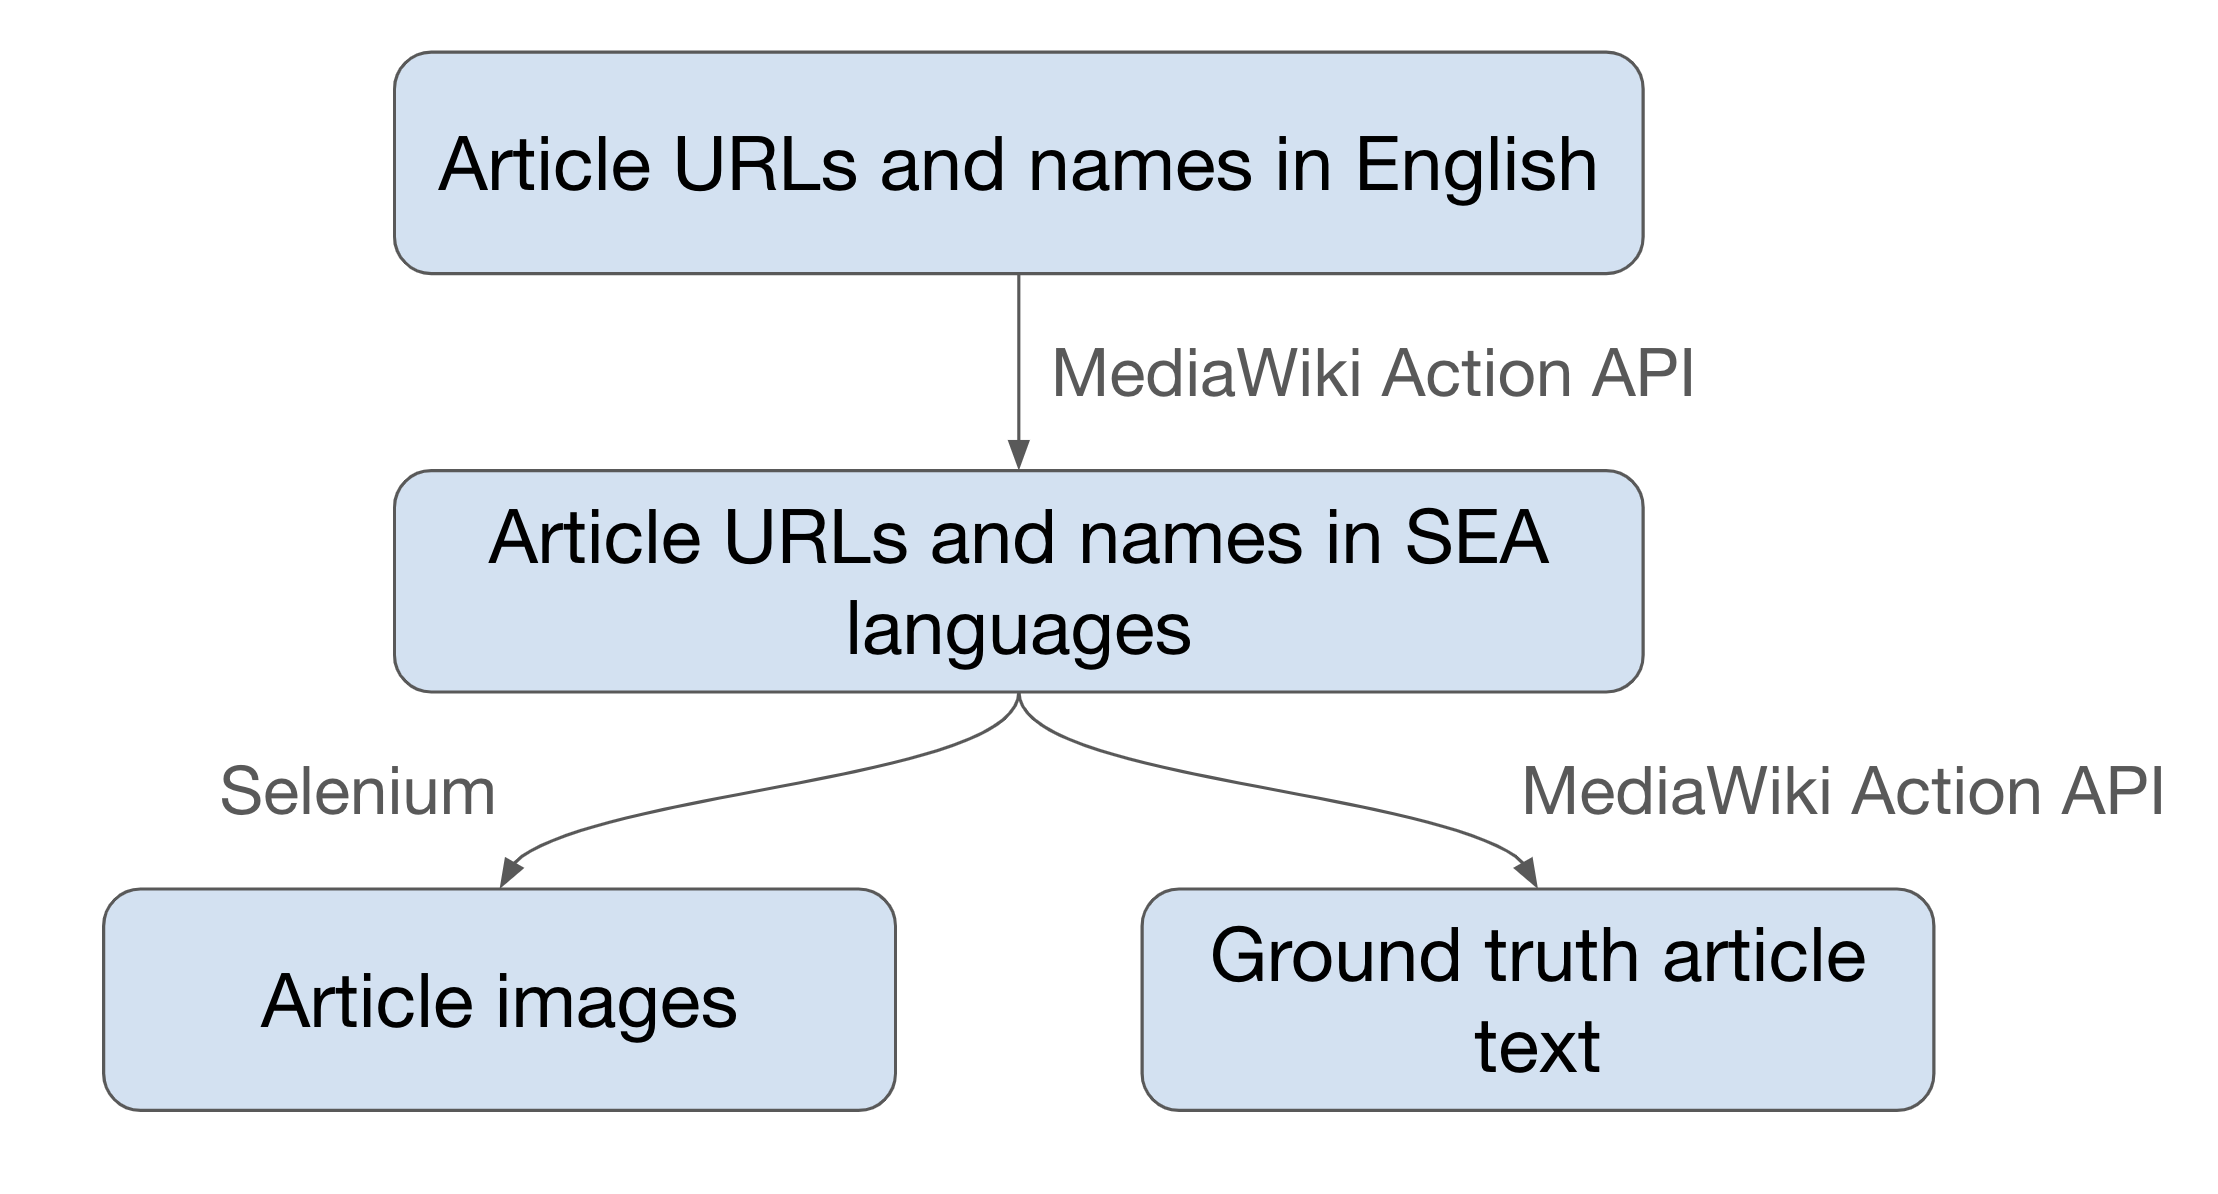
\includegraphics[width=0.6\textwidth]{images/data-collection.png}
    \caption{Pipeline for data collection from Wikipedia}
    \label{figure:data-collection}
\end{figure}

From the dataset of 100 Wikipedia articles, we collected article images and ground 
truth article text in our selected languages using Python, 
Selenium\footnote{\href{https://selenium-python.readthedocs.io}{Selenium} is a 
framework for automating web browsers, commonly used for web scraping by programmatically 
interacting with websites.}, and the MediaWiki Action API\footnote{The \href{https://www.mediawiki.org/wiki/API:Main_page}{MediaWiki Action API} allows 
access to wiki page operation features such as search and retrieval.}. Figure \ref{figure:data-collection} illustrates the overall pipeline 
for data collection. The detailed steps are as follows:

\begin{enumerate}
    \item Manually compile the dataset’s article names and URLs in English.
    \item Fetch the article names and URLs in Thai, Vietnamese, and Indonesian from the MediaWiki Action API.
    \item Download the article PDFs in all languages using Selenium.
    \item Convert the article PDFs into PNG images, where each image represents one page in the PDF.
    \item Download the ground truth article text into TXT files from the MediaWiki Action API.
\end{enumerate}

\section{Experiment 2: Benchmarking on Synthetic Data}

\subsection{Synthetic Data Generation}

\section{Experiment 3: Fine-tuning for Vietnamese and Thai}

\chapter{Results and Analysis}

In this chapter, we analyze and evaluate the results of the experiments to provide answers to the research questions.

\section{RQ1: How do popular OCR tools perform on SEA scripts?}

\subsection{OCR Accuracy}

\subsection{Runtime}

\begin{table}[ht]
    \caption{Average OCR runtime per page (seconds)}
    \label{table:runtime}
    \centering
    \begin{tabular}{lccc}
        \toprule
        & EasyOCR & Tesseract & GOT\\ 
        \midrule
        English & 3.23 & 11.68 & 24.35\\
        Indonesian & 2.92 & 13.19 & 31.44\\
        Vietnamese & 3.91 & 11.80 & -\\
        Thai & 2.32 & 16.76 & -\\
        \bottomrule
    \end{tabular}
\end{table}

\section{RQ2: What script-related challenges affect OCR accuracy on SEA languages?}

\begin{table}[ht]
    \caption{Error classification by character type for English articles}
    \label{table:english-error-classification}
    \centering
    \begin{tabular}{lrrrr}
        \toprule
        & \multirow{2}{*}{Count} & EasyOCR & Tesseract & GOT\\
        & & \% Missed & \% Missed & \% Missed\\
        \midrule
        Arabic digit & 38,324 & 0.7\% & 1.9\% & 0.3\%\\
        Latin letter & 1,546,964 & 1.3\% & 1.8\% & 0.4\%\\
        Latin letter w/ diacritic & 424 & 100.0\% & 53.1\% & 14.6\%\\
        Punctuation & 53,403 & 28.4\% & 2.3\% & 3.4\%\\
        Whitespace & 317,587 & 4.9\% & 4.3\% & 3.6\%\\
        Other & 3,298 & 82.8\% & 68.5\% & 76.9\%\\
        \bottomrule
    \end{tabular}
\end{table}

\begin{table}[ht]
    \caption{Error classification by character type for Indonesian articles}
    \label{table:indonesian-error-classification}
    \centering
    \begin{tabular}{lrrrr}
        \toprule
        & \multirow{2}{*}{Count} & EasyOCR & Tesseract & GOT\\
        & & \% Missed & \% Missed & \% Missed\\
        \midrule
        Arabic digit & 24,947 & 0.4\% & 1.8\% & 0.2\%\\
        Latin letter & 1,208,707 & 0.5\% & 1.8\% & 0.4\%\\
        Latin letter w/ diacritic & 262 & 5.3\% & 100.0\% & 15.3\%\\
        Punctuation & 37,788 & 22.1\% & 3.1\% & 0.8\%\\
        Whitespace & 207,556 & 4.8\% & 5.1\% & 4.1\%\\
        Other & 2,468 & 72.2\% & 80.5\% & 43.2\%\\
        \bottomrule
    \end{tabular}
\end{table}

\begin{table}[ht]
    \caption{Error classification by character type for Vietnamese articles}
    \label{table:vietnamese-error-classification}
    \centering
    \begin{tabular}{lrrr}
        \toprule
        & \multirow{2}{*}{Count} & EasyOCR & Tesseract\\
        & & \% Missed & \% Missed\\
        \midrule
        Arabic digit & 31,473 & 1.1\% & 2.2\%\\
        Latin letter & 916,667 & 8.5\% & 1.8\%\\
        Latin letter w/ diacritic & 292,686 & 14.8\% & 1.8\%\\
        Punctuation & 40,420 & 24.6\% & 2.2\%\\
        Whitespace & 367,936 & 10.9\% & 5.3\%\\
        Other & 35,767 & 12.5\% & 7.7\%\\
        \bottomrule
    \end{tabular}
\end{table}

\begin{table}[ht]
    \caption{Error classification by character type for Thai articles}
    \label{table:thai-error-classification}
    \centering
    \begin{tabular}{lrrr}
        \toprule
        & \multirow{2}{*}{Count} & EasyOCR & Tesseract\\
        & & \% Missed & \% Missed\\
        \midrule
        Arabic digit & 22,580 & 0.9\% & 6.7\%\\
        Latin letter & 36,174 & 100.0\% & 100.0\%\\
        Latin letter w/ diacritic & 96 & 100.0\% & 100.0\%\\
        Thai letter & 617,699 & 0.4\% & 3.1\%\\
        Thai diacritic & 90,620 & 3.7\% & 3.6\%\\
        Punctuation & 13,669 & 6.4\% & 8.4\%\\
        Thai punctuation & 901 & 78.8\% & 3.9\%\\
        Whitespace & 58,164 & 37.5\% & 37.2\%\\
        Other & 306,647 & 2.2\% & 7.1\%\\
        \bottomrule
    \end{tabular}
\end{table}

\section{RQ3: What techniques and recommendations can enhance OCR accuracy on SEA languages?}

\chapter{Discussion}

\chapter{Conclusion}

\printbibliography[title={References}]

\clearpage
\appendix
\renewcommand{\chaptername}{Appendix}

\chapter{Wikipedia Article Dataset}

\begin{table}[ht]
    \centering
    \begin{tabular}{p{1in}p{3.8in}}
        \toprule
        \textbf{Category} & \textbf{Articles} \\
        \midrule
        People & Elizabeth II, Barack Obama, Michael Jackson, Elon Musk, Lady Gaga, Adolf Hitler, Eminem, Lionel Messi, Justin Bieber, Freddie Mercury, Kim Kardashian, Johnny Depp, Steve Jobs, Dwayne Johnson, Michael Jordan, Taylor Swift, Stephen Hawking, Kanye West, Donald Trump\\
        \midrule
        Present countries & United States, India, United Kingdom, Canada, Australia, China, Russia, Japan, Germany, France, Singapore, Israel, Pakistan, Philippines, Brazil, Italy, Netherlands, New Zealand, Ukraine, Spain\\
        \midrule
        Cities & New York City, London, Hong Kong, Los Angeles, Dubai, Washington, D.C., Paris, Chicago, Mumbai, San Francisco, Rome, Monaco, Toronto, Tokyo, Philadelphia, Machu Picchu, Jerusalem, Amsterdam, Boston\\
        \midrule
        Life & Cat, Dog, Animal, Lion, Coronavirus, Tiger, Human, Dinosaur, Elephant, Virus, Horse, Photosynthesis, Evolution, Apple, Bird, Mammal, Potato, Polar bear, Shark, Snake\\
        \midrule
        Buildings and structures & Taj Mahal, Burj Khalifa, Statue of Liberty, Great Wall of China, Eiffel Tower, Berlin Wall, Stonehenge, Mount Rushmore, Colosseum, Auschwitz concentration camp, Great Pyramid of Giza, One World Trade Center, Empire State Building, White House, Petra, Large Hadron Collider, Hagia Sophia, Golden Gate Bridge, Panama Canal, Angkor Wat\\
        \bottomrule
    \end{tabular}
    \caption{Dataset of 98 Wikipedia articles}
    \label{table:dataset}
\end{table}

\end{document}
